\documentclass[tikz]{standalone}
\usepackage{pgfplots}
%\pgfplotsset{compat=1.8}
\begin{document}
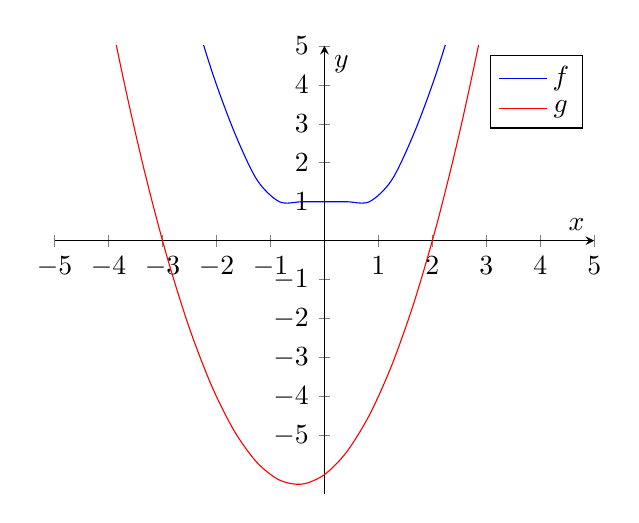
\begin{tikzpicture}[
    declare function={
      func(\x)= (\x<=-1) * (\x*\x)   +
      and(\x>=-1, \x<=1) * (1)     +
      (\x>=1) * (\x*\x);
      g(\x)= \x*\x + \x - 6;
    }
  ]
  \begin{axis}[
      axis x line=middle, axis y line=middle,
      ymin=-6.5, ymax=5, ytick={-5,...,5}, ylabel=$y$,
      xmin=-5, xmax=5, xtick={-5,...,5}, xlabel=$x$,
    ]
    \addplot[blue, domain=-5:5, smooth]{func(x)} node [pos=0.75,pin={-10:$x^2$},inner sep=0pt] {};
    \addplot[red, domain=-5:5, smooth]{g(x)}node [pos=0.75,pin={-10:$x^2$},inner sep=0pt] {};
    \legend{$f$,$g$}
  \end{axis}
\end{tikzpicture}
\end{document}
